\section{Software Design}

\subsection{Global C Function parameterize()}

This package's entry point is:

\begin{ccExampleCode}

// Compute a 1 to 1 mapping from a triangular 3D surface 'mesh' to 2D circle,
// using Floater's mean value coordinates algorithm.
// 1 to 1 mapping is guaranteed.
template <class MeshAdaptor_3>
typename Parametizer_traits_3<MeshAdaptor_3>::Error_code
parameterize(MeshAdaptor_3* mesh)
{
    Mean_value_coordinates_parametizer_3<MeshAdaptor_3> parametizer;
    return parametizer.parameterize(mesh);
}

// Compute a 1 to 1 mapping from a triangular 3D surface 'mesh'
// to a piece of the 2D space.
// 1 to 1 mapping may be guaranteed or not, depending of
// ParametizerTraits_3 algorithm chosen.
template <class MeshAdaptor_3, class ParametizerTraits_3>
typename Parametizer_traits_3<MeshAdaptor_3>::Error_code
parameterize(MeshAdaptor_3* mesh,
             ParametizerTraits_3 parametizer)
{
    return parametizer.parameterize(mesh);
}

\end{ccExampleCode}

You may notice that these global functions simply call the
parameterize() method of a ParametizerTraits\_3 object.
The purpose of these global functions is:
\begin{itemize}
\item to be consistent with other CGAL algorithms that are also provided as
      global functions, e.g. convex\_hull\_2()
\item to provide a default parameterization method (Floater's mean value coordinates),
      which wouldn't be possible with a direct call to an object's method
\end{itemize}

You may also wonder why there is not just one parameterize() function with a
default ParametizerTraits\_3 argument equal to
Mean\_value\_coordinates\_parametizer\_3$<$MeshAdaptor\_3$>$.
The reason is simply that this is not allowed by the C++ standard (see
\cite{cgal:ansi-is14882-98}, paragraph 14.1/9).


\subsection{ParametizerTraits\_3 is not a Traits Class}

In this package, we focus on triangulated surfaces that are homeomorphic to a
disk and on piecewise linear mappings into a planar domain.
A consequence is that the skeleton of all parameterization methods of this
package is the same:
\begin{itemize}
\item Allocate a sparse linear system A*X = B
\item Parameterize the mesh boundary and initialize B
\item Parameterize the inner points of the mesh and set A coefficients
\item Solve the system
\end{itemize}

It is tempting to make the parameterization method a traits class that
modifies the behavior of a common parameterization algorithm.

In the other hand, there are several differences among methods:
\begin{itemize}
\item Fixed border methods need to parameterize all boundary vertices,
      when free border methods parameterize only two vertices
\item Some methods create symmetric definite positive systems,
      which may be solved more efficiently that general systems
\item Most parameterization methods use two \#vertices x \#vertices systems,
      when LSCM uses one (2 * \#triangles) x \#vertices system
\item Most parameterization methods invert the A matrix,
      when LSCM solves the system in the least squares sense
\end{itemize}

The software design chosen is:
\begin{itemize}
\item Each ParametizerTraits\_3 class has template arguments
      defining the border parameterization and sparse linear solver to use,
      with default values adapted to the method
\item Each ParametizerTraits\_3 class implements its own version
      of the parameterization algorithm as a parameterize() method
\item Code factorization is achieved using a class hierarchy
\end{itemize}

% Include parametizer_class_diagram.png/eps figure
\begin{figure}[bht]
    \begin{center}
        % Image
        \begin{ccTexOnly}
            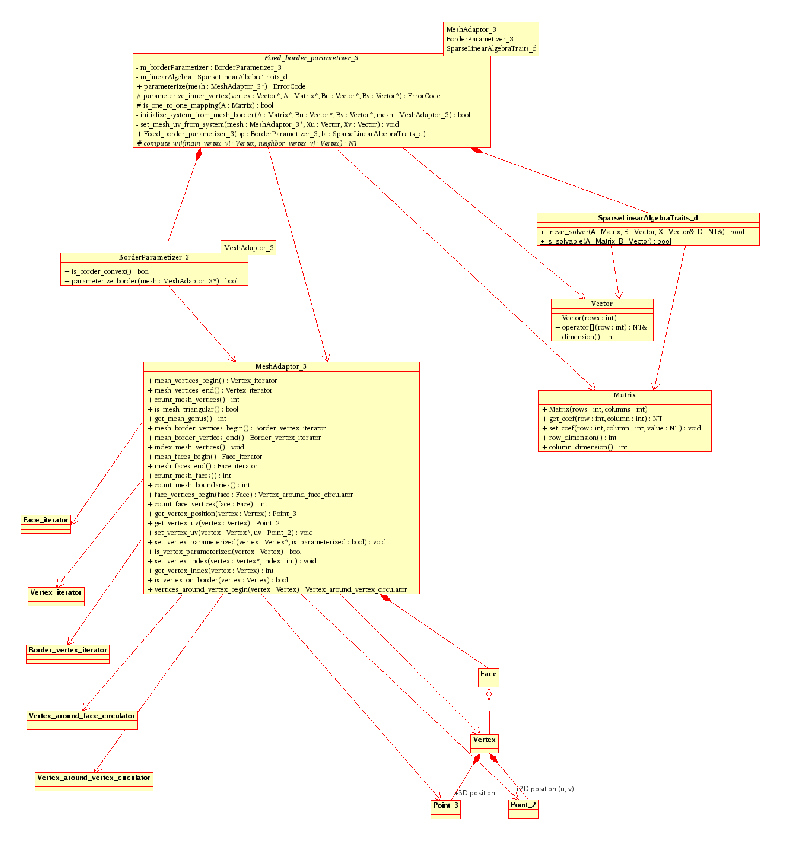
\includegraphics{Parameterization/parametizer_class_diagram}
        \end{ccTexOnly}
        \begin{ccHtmlOnly}
            <img border=0 src="./parametizer_class_diagram.png" align=center WIDTH="80%">
        \end{ccHtmlOnly}
        \label{parameterization-fig-parametizer_class_diagram}

        % Title
        \caption{A parametizer's UML class diagram (main types and methods only)}
    \end{center}
\end{figure}

% Include parametizers_class_hierarchy.png/eps figure
\begin{figure}[bht]
    \begin{center}
        % Image
        \begin{ccTexOnly}
            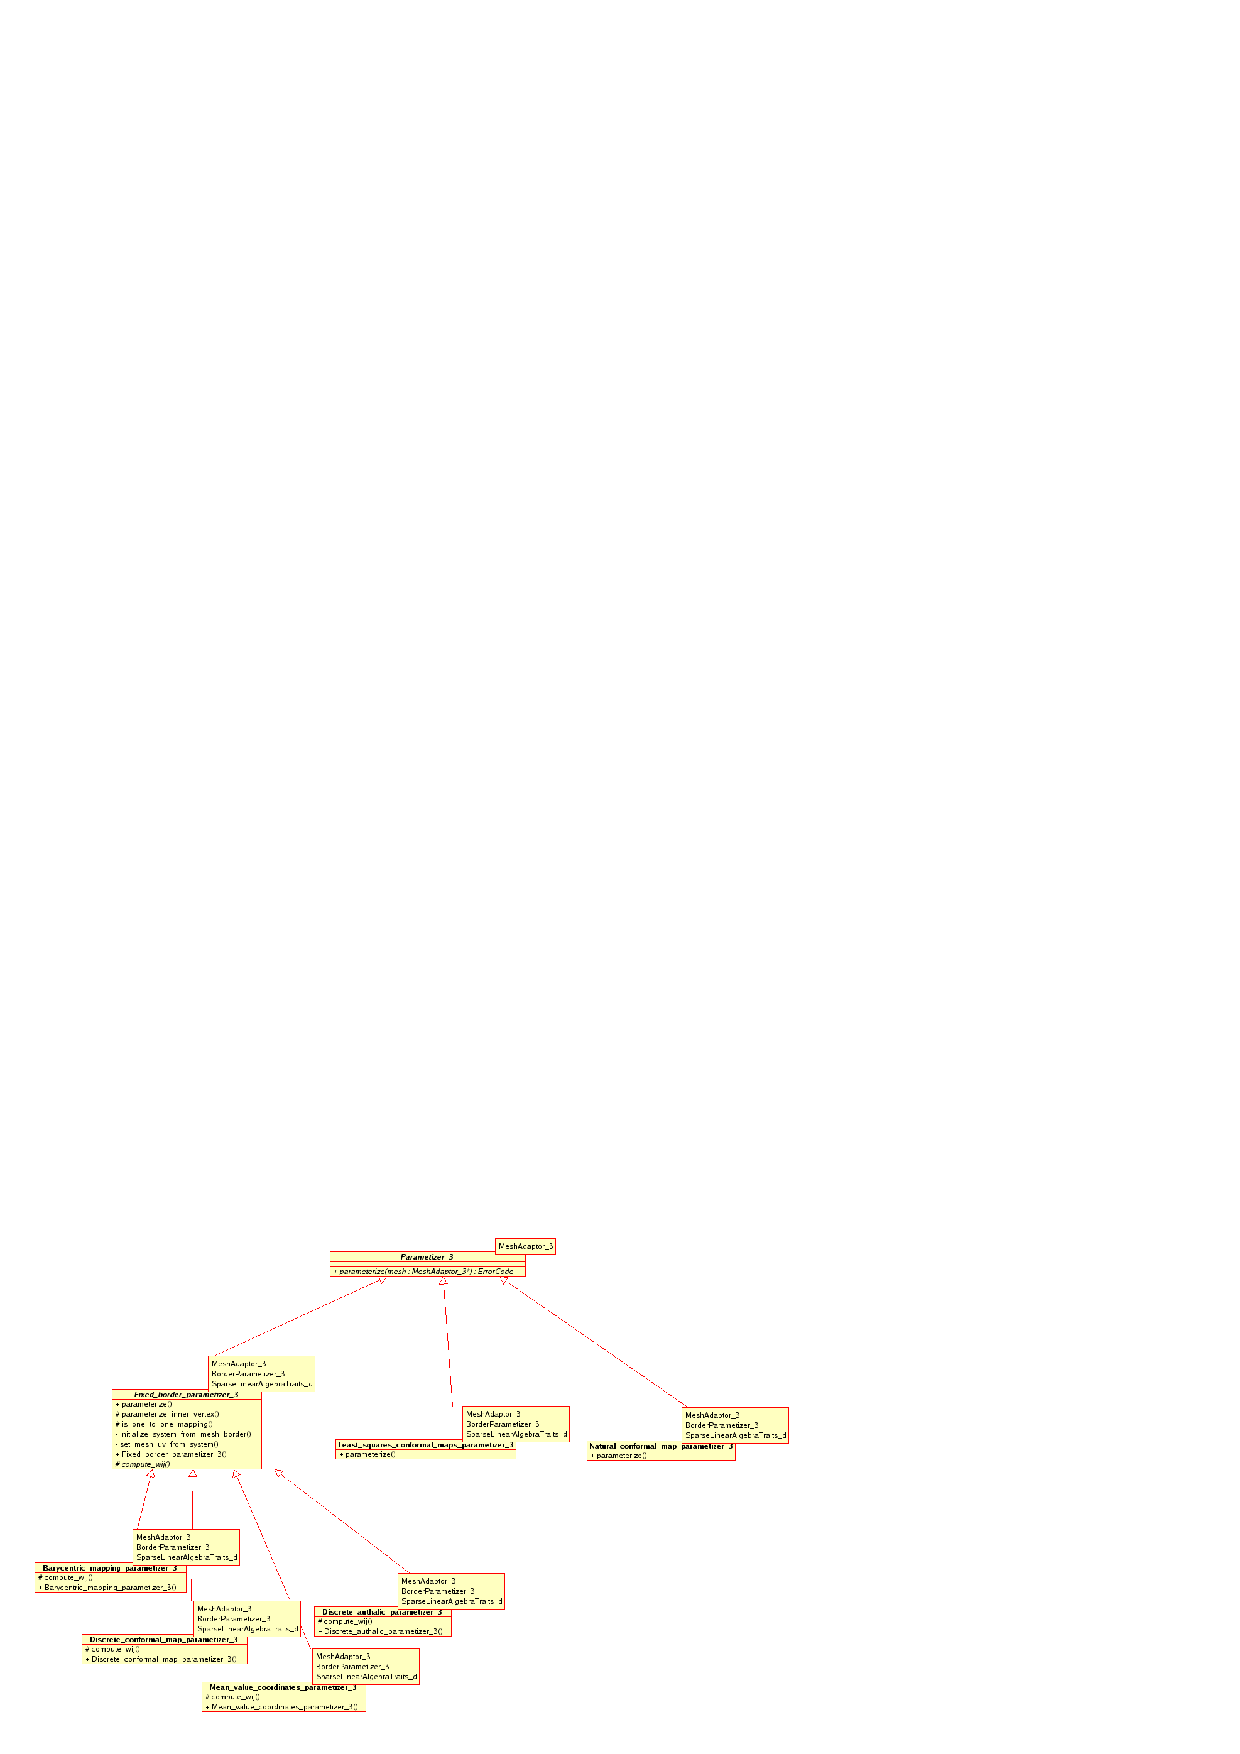
\includegraphics{Parameterization/parametizers_class_hierarchy}
        \end{ccTexOnly}
        \begin{ccHtmlOnly}
            <img border=0 src="./parametizers_class_hierarchy.png" align=center WIDTH="80%">
        \end{ccHtmlOnly}
        \label{parameterization-fig-parametizers_class_hierarchy}

        % Title
        \caption{Parametizers class hierarchy}
    \end{center}
\end{figure}


\subsection{Fixed\_border\_parametizer\_3 Class}

Linear fixed border parameterization algorithms are very close. They mainly
differ by the energy that they try to minimize, i.e. by the value of the $wij$
coefficient of the A matrix, for $vi$ and $vj$ neighbor vertices of the mesh.
See details in \cite{cgal:fh-survey-05}.

The consequence is that most of the code of the fixed border methods
is factorized in the Fixed\_border\_parametizer\_3 class.
Subclasses:
\begin{itemize}
\item must provide BorderParametizer\_3 and SparseLinearAlgebraTraits\_d template parameters that make sense
\item must implement compute\_wij() to compute $wij$ = (i,j) coefficient of matrix A for $vj$ neighbor vertex of $vi$
\item may implement a optimized version of is\_one\_to\_one\_mapping()
\end{itemize}

See Barycentric\_mapping\_parametizer\_3 example.


\subsection{Boundary Parameterizations}

Boundary Parameterizations are models of the BorderParametizer\_3 concept.

To simplify the implementation, BorderParametizer\_3 models know only the
MeshAdaptor\_3 mesh class. They don't know the parameterization algorithm
nor the sparse linear solver used.


\subsection{MeshAdaptor\_3 and PatchableMeshAdaptor\_3 Concepts}

All parameterization methods are templated by the kind of mesh they are applied on.
The mesh type must be a model of MeshAdaptor\_3.

The purpose of such a model is to:
\begin{itemize}
\item a) Support several kind of meshes
\item b) Hide the implementation of extra fields specific to the parameterization domain
      (index, u, v, is\_parameterized)
\item c) Handle in the mesh type the complexity of virtually "cutting" a mesh
      to make it homeomorphic to a disk (instead of duplicating this
      code in each parameterization method)
\end{itemize}

Two options are possible for a) and b):
\begin{itemize}
\item Pass to all classes and methods a mesh pointer, a traits class to manipulate it,
      and accessors to the extra fields arrays.
      This is the choice of the Boost Graph Library with boost::graph\_traits$<>$
      and the property maps.
\item Pass to all classes and methods an object that points to the actual mesh and knows
      how to access to it. This is the Adaptor concept described in
      \cite{cgal:ghjv-dpero-95}.
\end{itemize}

The current design of this package uses the second option, which is simpler.
Of course, we may decide to switch to the first one to reach a deeper integration
of CGAL with Boost.

Point c) is solved by class Mesh\_adaptor\_patch\_3, which takes care
of virtually "cutting"
a patch in a PatchableMeshAdaptor\_3 mesh, to make it appear as a topological disk
with a MeshAdaptor\_3 interface.
PatchableMeshAdaptor\_3 inherits from concept MeshAdaptor\_3 and adds
the ability to support patches and virtual seams.
This mainly means that:
\begin{itemize}
\item vertices can be tagged as inside or outside the patch to parameterize
\item the fields specific to parameterizations (index, u, v, is\_parameterized)
      can be set per "corner" (aka half-edge)
\end{itemize}


\subsection{SparseLinearAlgebraTraits\_d Concept}

This package solves sparse linear systems using solvers which are models
of SparseLinearAlgebraTraits\_d.

SparseLinearAlgebraTraits\_d is a sub-concept of LinearAlgebraTraits\_d concept
in Kernel\_d.
The goal is to adapt easily code wriiten for dense matrices to sparse ones,
and vice-versa.


\subsection{Cutting a Mesh}

In this package, we focus on triangulated surfaces that are homeomorphic to a
disk.

Computing a cut that transforms
a closed mesh of arbitrary genus into a topological disk is a research domain
of its own. This package doesn't cover this subject.



